% 
% Interface
% @author Pieter Maene <pieter.maene@student.kuleuven.be>
%

\chapter{Interface}
\label{chap:interface}

Het verbeteren van de gebruiksvriendelijkheid van het Helios verkiezingssysteem was een belangrijk doel van deze thesis. Er zijn op vier belangrijke plaatsen wijzigingen aangebracht. Veruit het meeste werk was nodig om de procedure (\ref{chap:procedure}) duidelijker te maken in het beheer (\ref{sec:ui:beheer}). Ook de gebruiksvriendelijkheid van het trustee dashboard werd sterk verbeterd (\ref{sec:ui:trustee_dashboard}). Tot slot werd ook de output van de applicatie die gebruikt kan worden om het resultaat te controleren, verduidelijkt (\ref{sec:ui:controleapplicatie}). Hoewel in dit hoofdstuk alleen de grootste aanpassingen besproken worden, werd de layout doorheen het hele systeem geüniformeerd.

\section{Beheer}
\label{sec:ui:beheer}

In de oude interface zaten het beheer en het bekijken van de verkiezing op dezelfde pagina (\ref{fig:kv:elections_view_old}). De gewone kiezers zagen de beheersfuncties uiteraard niet, maar dit maakte het wel ingewikkeld voor de beheerder. Bovendien was het niet duidelijk wat de volgende stap was of waar de beheerder juist in de procedure zat. Daarom werd besloten om deze twee functies uit elkaar te halen en een aparte pagina te voorzien voor het beheer (\ref{fig:kv:elections_admin}).

\npar Op deze nieuwe pagina wordt de volledige procedure weergegeven. Er wordt ook aangegeven wat de volgende stap is en welke stappen reeds allemaal voltooid zijn. Tot slot staan onderaan alle problemen die nog opgelost moeten worden voordat het stembiljet bevroren kan worden.

%TODO Referentie naar Threshold Encryptie in Helios

\npar Voor een verkiezing met threshold encryptie zijn er belangrijke veranderingen in de workflow. Robbert Coeckelbergh had een publiek bulletin board ge\"introduceerd waar iedereen sleutelparen voor communicatie kon aanmaken en uploaden. De beheerder kon dan trustees toevoegen aan een verkiezing door ze te selecteren uit een lijst. Dit betekent ook dat dezelfde sleutelparen voor communicatie gebruikt werden bij elke verkiezing waar deze persoon trustee was.

\npar Voordat alle trustees toegevoegd konden worden aan een trustee, moest de beheerder dus wachten totdat iedereen zijn sleutelparen voor communicatie ge\"upload had. Omdat iedereen hiervoor buiten het systeem om nog eens gecontacteerd moest worden, maakte dit de sleutelceremonie nog ingewikkelder. Daarom werd besloten om het bulletin board weg te halen. De trustees worden nu eerst toegevoegd aan de verkiezing, waarna ze een link krijgen toegestuurd naar hun trustee dashboard (\ref{sec:ui:trustee_dashboard}). De eerst stap van de sleutelceremonie die ze daar moeten uitvoeren, is nu het uploaden van de sleutelparen voor communicatie.

\begin{figure}
  \center{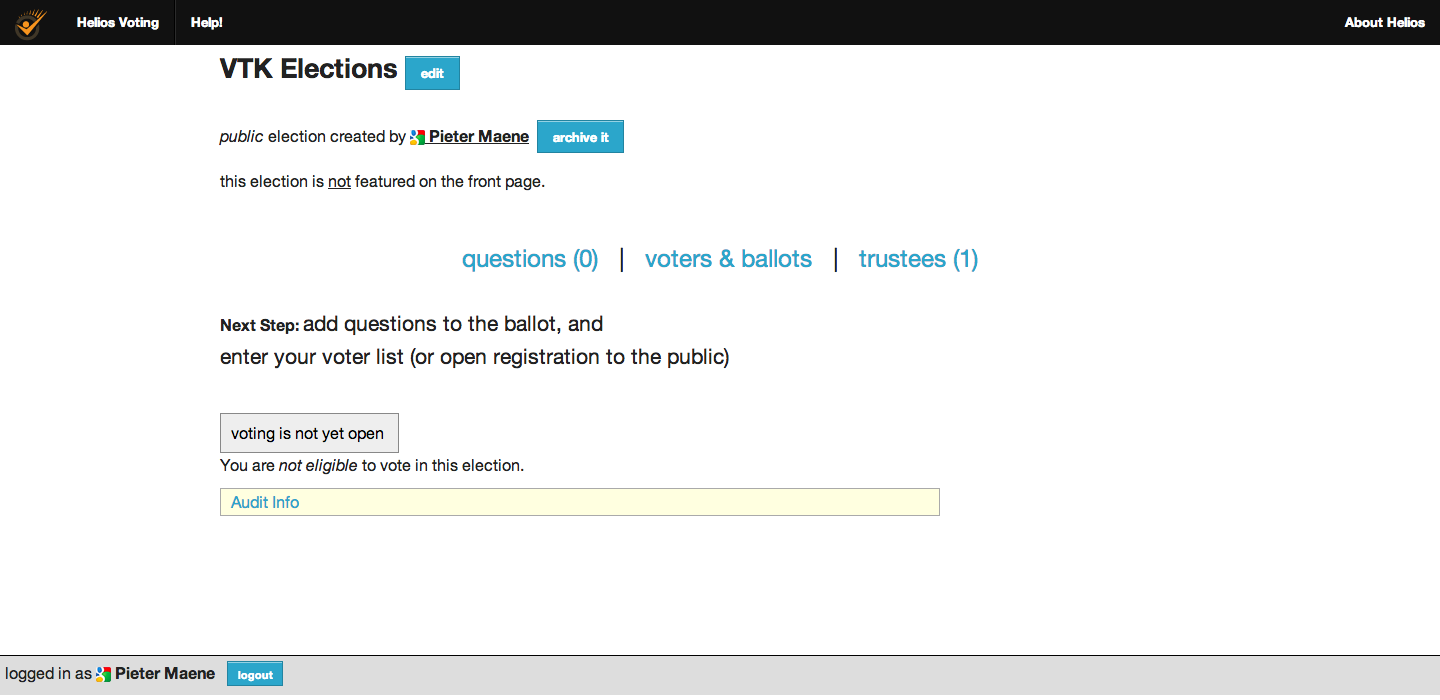
\includegraphics[width=\linewidth]{ui/elections_view_old.png}}
  \caption{Overzicht van de verkiezing (oud)}
  \label{fig:kv:elections_view_old}
\end{figure}

\begin{figure}
  \center{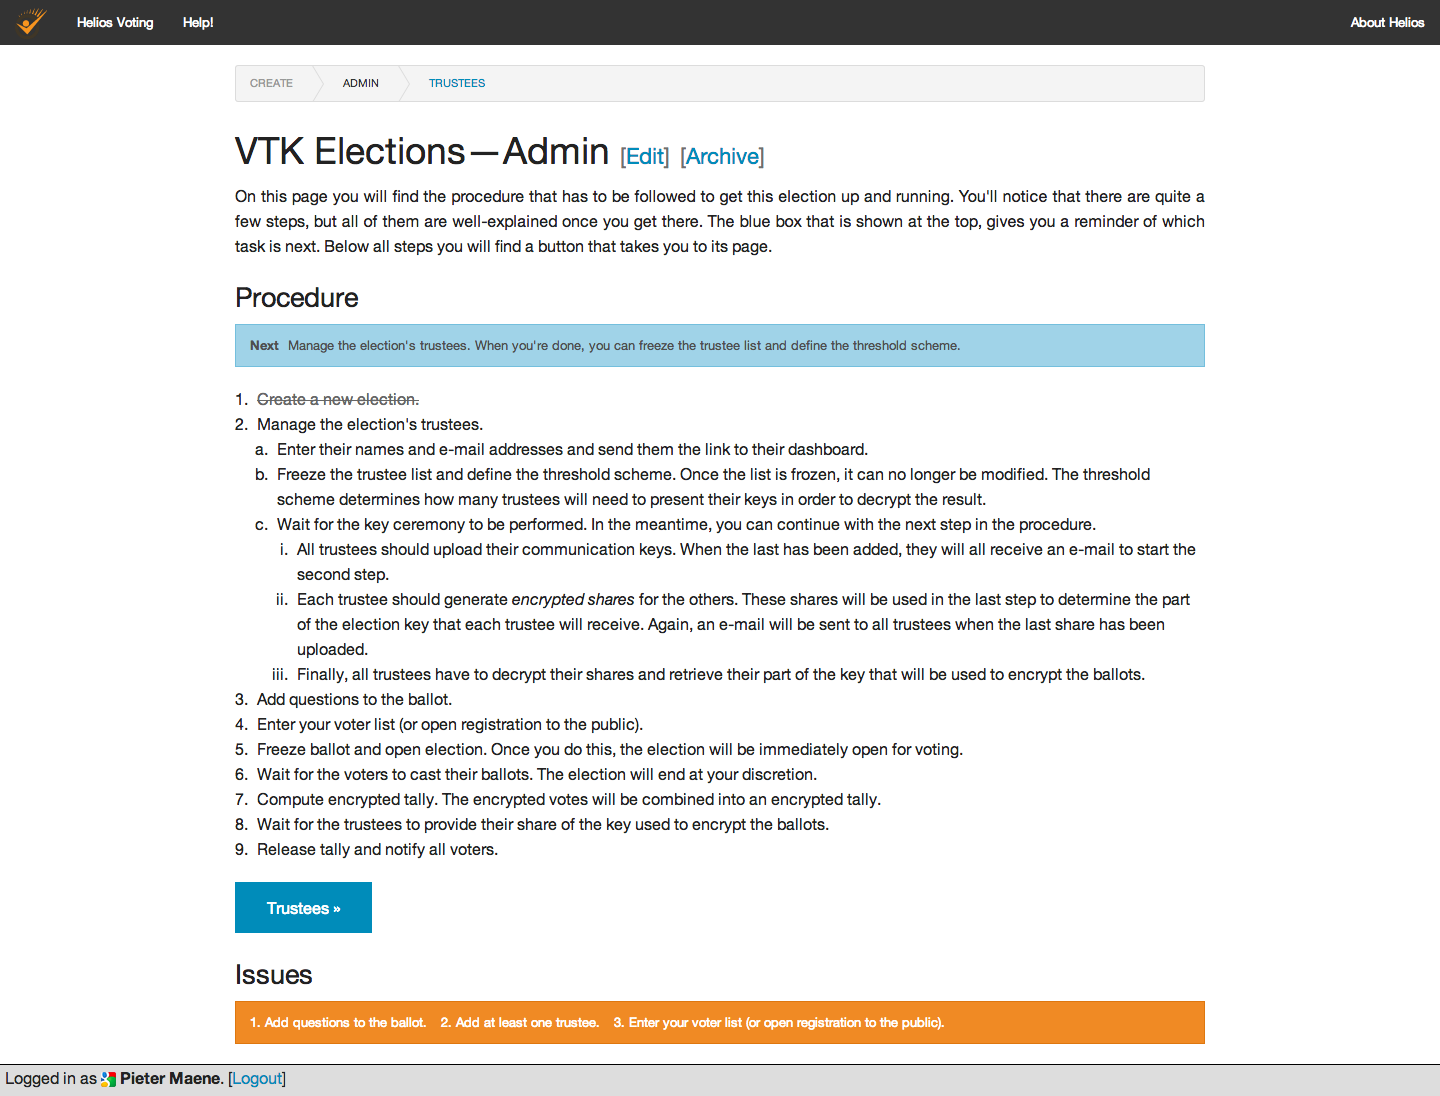
\includegraphics[width=\linewidth]{ui/elections_admin.png}}
  \caption{Beheer van de verkiezing}
  \label{fig:kv:elections_admin}
\end{figure}

\section{Trustee Dashboard}
\label{sec:ui:trustee_dashboard}



\section{Controleapplicatie}
\label{sec:ui:controleapplicatie}
